\subsubsection{Interrupts from the Pushbutton Keys}

Figure \ref{fig:pushbutton_port}, reproduced as Figure \ref{fig:pushbutton_port_int},
shows the registers associated with the pushbutton parallel port. 
The {\it Interruptmask} register allows processor interrupts to be generated when a key is
pressed.  Each bit in the {\it Edgecapture} register is set to 1 by the parallel port when the
corresponding key is pressed. The processor can read this register
to determine which key has been pressed, in addition to receiving an interrupt request if the
corresponding bit in the {\it Interruptmask} register is set to 1. Writing a 1 into a bit position
in the {\it Edgecapture} register clears the bit to 0 and deasserts the interrupt request.

\begin{figure}[h!]
   \begin{center}
       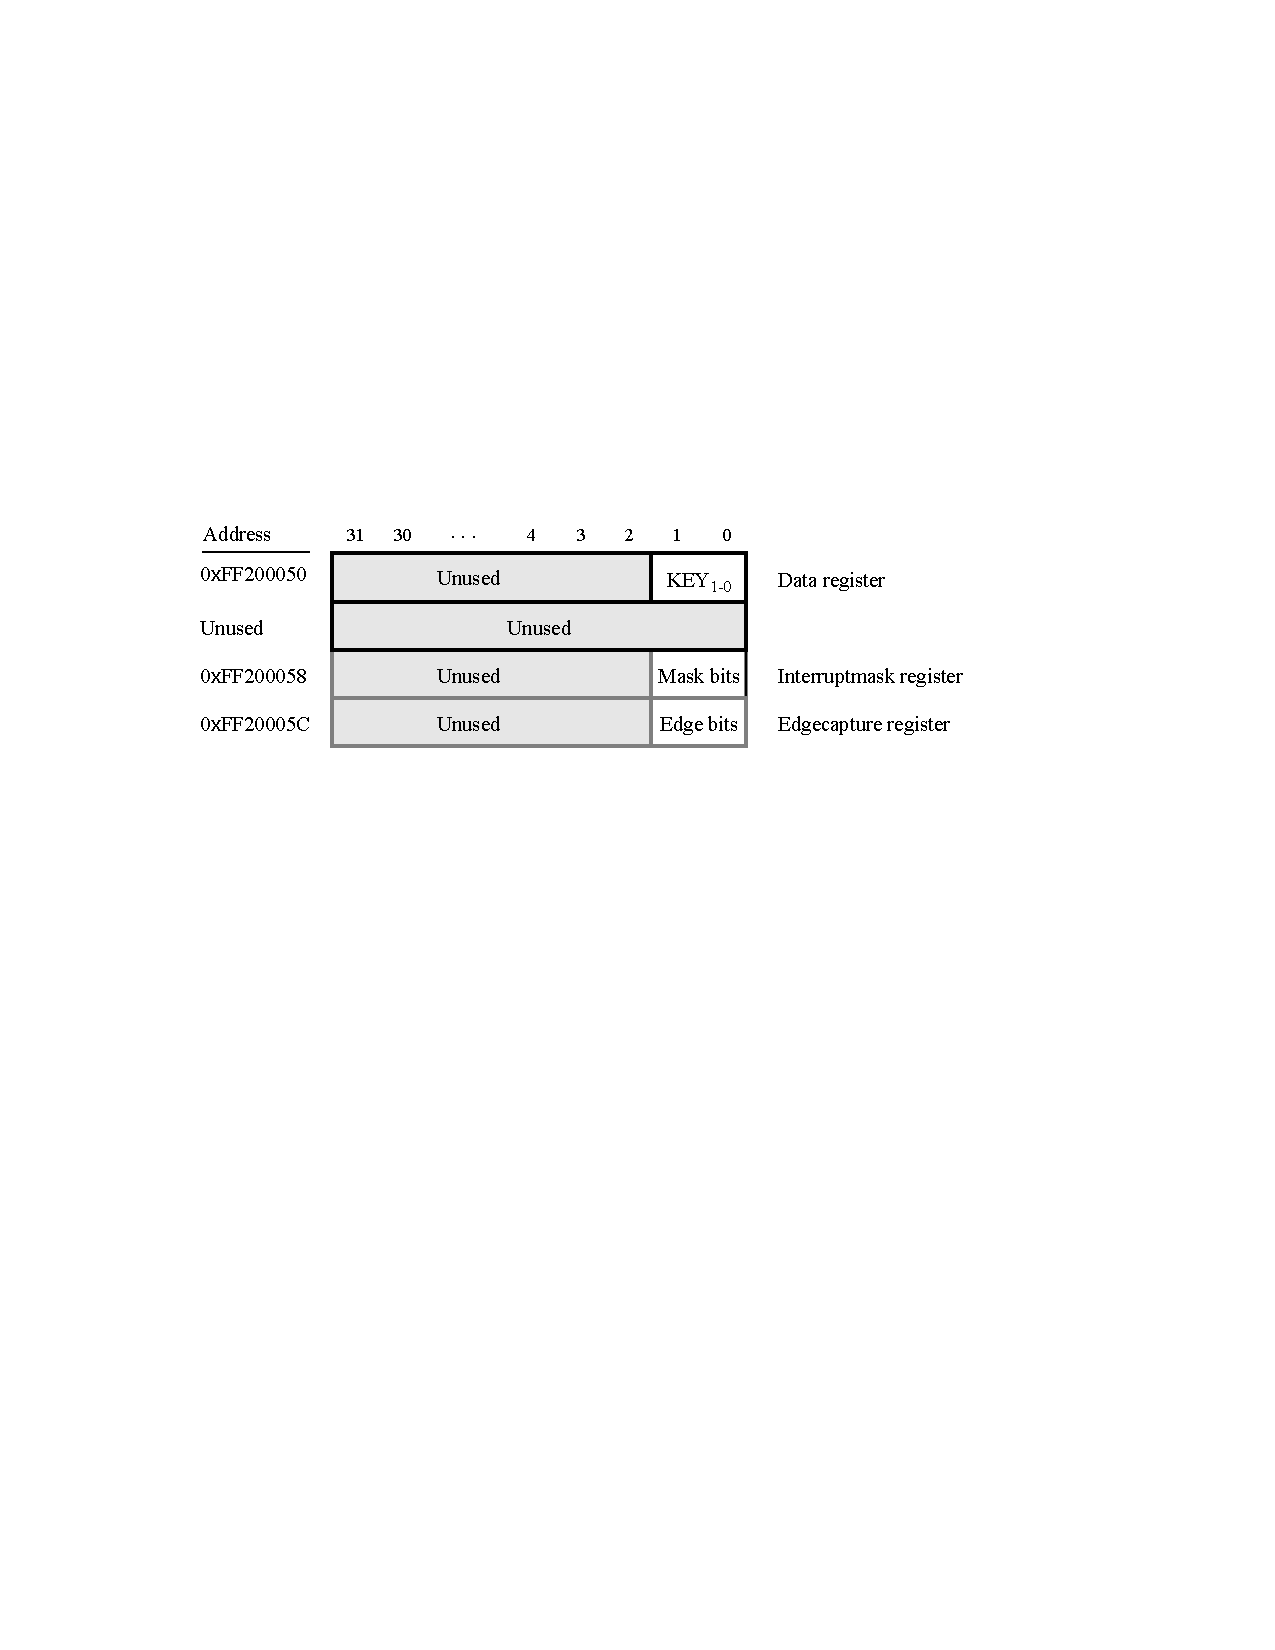
\includegraphics{../../../common/figs/FPGA_PP_Keys_2.pdf}
   \end{center}
   \caption{Registers used for interrupts from the pushbutton parallel port.}
	\label{fig:pushbutton_port_int}
\end{figure}